%  Worked example for the axioms-paper-format skill: a complete Axioms manuscript on the
%  official MDPI class. Authors, affiliations, e-mails and ORCID iDs are FICTIONAL
%  placeholders. The mathematics is elementary but correct; the references are real
%  publications -- verify every entry before reusing it. Copy, then replace everything.
%=================================================================
\documentclass[axioms,article,submit,moreauthors]{Definitions/mdpi}

%=================================================================
% MDPI internal commands - do not modify
\firstpage{1}
\makeatletter
\setcounter{page}{\@firstpage}
\makeatother
\pubvolume{1}
\issuenum{1}
\articlenumber{0}
\pubyear{2026}
\copyrightyear{2026}
\datereceived{ }
\daterevised{ } % Comment out if no revised date
\dateaccepted{ }
\datepublished{ }

%=================================================================
% Own macros (the class already loads amsmath, amssymb, amsthm, graphicx, booktabs, ...)
\newcommand{\N}{\mathbb{N}}
\newcommand{\R}{\mathbb{R}}

%=================================================================
\Title{An A Priori Error Bound for Picard Iterations of Contractions on Complete Metric Spaces}

\newcommand{\orcidauthorA}{0000-0002-1825-0097} % fictional (ORCID's own documentation example)

\Author{Ivan Petrenko $^{1}$\orcidA{} and Olena Kovalenko $^{2,}$*}

\AuthorNames{Ivan Petrenko and Olena Kovalenko}

\address{%
$^{1}$ \quad Department of Mathematical Methods of System Analysis, Igor Sikorsky Kyiv Polytechnic Institute, 03056 Kyiv, Ukraine; i.petrenko@example.com\\
$^{2}$ \quad Department of Applied Mathematics, Example University, 79000 Lviv, Ukraine; o.kovalenko@example.com}

\corres{Correspondence: o.kovalenko@example.com}

\abstract{Fixed point iterations are the standard constructive tool for proving existence and uniqueness of solutions of nonlinear equations, and practical computations need an explicit stopping rule that does not depend on the unknown fixed point. This note revisits the Banach contraction principle on a complete metric space and gives a self-contained proof of the a priori error bound for Picard iterations, which estimates the distance between the $n$-th iterate and the fixed point through the contraction constant and the first step only. The proof uses a telescoping estimate for consecutive iterates and the completeness of the space. The bound is sharp up to a constant factor for the scalar map $x\mapsto \tfrac12\cos x$, for which we compare the computed errors with the estimate and derive the number of iterations that guarantees a prescribed accuracy. The result yields a stopping criterion that can be evaluated before the iteration starts, and it extends verbatim to every closed subset of a Banach space that is mapped into itself by a contraction.}

\keyword{Banach contraction principle; fixed point; Picard iteration; a priori estimate; complete metric space}

\MSC{47H10; 54H25; 65J15}

%%%%%%%%%%%%%%%%%%%%%%%%%%%%%%%%%%%%%%%%%%
\begin{document}

\section{Introduction}

The contraction mapping principle of Banach~\cite{banach1922} is the prototype of a constructive fixed point theorem: a contraction of a complete metric space has exactly one fixed point, and the Picard iterates converge to it from every starting point. Its many generalisations, for example to Caristi-type maps~\cite{caristi1976}, to contractive maps on compact spaces~\cite{edelstein1962} and to nonexpansive maps~\cite{kirk1965}, are surveyed in the monographs~\cite{goebel1990,granas2003}.

For computations, the decisive question is when to stop the iteration. Ref.~\cite{granas2003} gives the classical answer in terms of the first step of the iteration; this note gives a short self-contained proof of that a priori estimate (Theorem~\ref{thm:apriori}) and illustrates its sharpness on a scalar example (Example~\ref{ex:cos}).

The rest of this paper is organized as follows. Section~\ref{sec:prelim} recalls the definitions and proves an estimate for consecutive iterates. Section~\ref{sec:main} states and proves the main result and discusses the example. Section~\ref{sec:concl} concludes the paper.

\section{Preliminaries}\label{sec:prelim}

Throughout, $(X,d)$ is a complete metric space.

\begin{Definition}\label{def:contraction}
A map $T\colon X\to X$ is a \emph{contraction} if there is $q\in[0,1)$ such that
\begin{equation}\label{eq:contraction}
d(Tx,Ty)\le q\,d(x,y)\quad\text{for all } x,y\in X.
\end{equation}
\end{Definition}

For $x_0\in X$ the \emph{Picard iterates} are $x_{n+1}=Tx_n$, $n\in\N\cup\{0\}$.

\begin{Lemma}\label{lem:steps}
If $T$ satisfies~\eqref{eq:contraction}, then $d(x_n,x_{n+1})\le q^n d(x_0,x_1)$ for every $n\ge 0$.
\end{Lemma}

\begin{proof}
The case $n=0$ is trivial. If the claim holds for $n$, then by~\eqref{eq:contraction}
\begin{equation}\label{eq:induction}
d(x_{n+1},x_{n+2})=d(Tx_n,Tx_{n+1})\le q\,d(x_n,x_{n+1})\le q^{n+1}d(x_0,x_1),
\end{equation}
which completes the induction.
\end{proof}

\section{Main Result}\label{sec:main}

\begin{Theorem}\label{thm:apriori}
Let $T\colon X\to X$ be a contraction with constant $q\in[0,1)$. Then $T$ has a unique fixed point $x^*$, and for every $x_0\in X$ and $n\ge 0$,
\begin{equation}\label{eq:apriori}
d(x_n,x^*)\le \frac{q^n}{1-q}\,d(x_0,x_1).
\end{equation}
\end{Theorem}

\begin{proof}
For $m>n$, the triangle inequality and Lemma~\ref{lem:steps} give
\begin{equation}\label{eq:cauchy}
d(x_n,x_m)\le\sum_{k=n}^{m-1}d(x_k,x_{k+1})\le d(x_0,x_1)\sum_{k=n}^{\infty}q^k=\frac{q^n}{1-q}\,d(x_0,x_1).
\end{equation}
Hence $(x_n)$ is a Cauchy sequence and converges to some $x^*\in X$ by completeness. Since $T$ is continuous, $x^*=\lim x_{n+1}=\lim Tx_n=Tx^*$. If also $Ty=y$, then $d(x^*,y)\le q\,d(x^*,y)$, so $y=x^*$. Letting $m\to\infty$ in~\eqref{eq:cauchy} yields~\eqref{eq:apriori}.
\end{proof}

\begin{Corollary}\label{cor:steps}
If $d(x_0,x_1)>0$ and $\varepsilon>0$, then $d(x_n,x^*)\le\varepsilon$ for every
\begin{equation}\label{eq:nsteps}
n\ge \frac{\ln\bigl(\varepsilon(1-q)/d(x_0,x_1)\bigr)}{\ln q}.
\end{equation}
\end{Corollary}

\begin{proof}
Inequality~\eqref{eq:nsteps} is equivalent to $q^n d(x_0,x_1)/(1-q)\le\varepsilon$; apply Theorem~\ref{thm:apriori}.
\end{proof}

\begin{Example}\label{ex:cos}
Let $X=\R$ and $Tx=\tfrac12\cos x$. By the mean value theorem, $|Tx-Ty|\le\tfrac12|x-y|$, so $q=\tfrac12$. With $x_0=0$, we have $x_1=\tfrac12$ and~\eqref{eq:apriori} reads $|x_n-x^*|\le 2^{-n}$. Table~\ref{tab:iterates} and Figure~\ref{fig:error} compare this bound with the actual error, where $x^*\approx 0.450184$; by~\eqref{eq:nsteps}, $n=20$ iterations guarantee $\varepsilon=10^{-6}$.
\end{Example}

\begin{table}[H]
\caption{Picard iterates of $Tx=\tfrac12\cos x$ from $x_0=0$, their error and the bound~\eqref{eq:apriori}.\label{tab:iterates}}
\begin{tabularx}{\textwidth}{CCCC}
\toprule
$\boldsymbol{n}$ & $\boldsymbol{x_n}$ & $\boldsymbol{|x_n-x^*|}$ & \textbf{Bound} $\boldsymbol{2^{-n}}$\\
\midrule
0 & 0.000000 & $4.50\times10^{-1}$ & 1.000000\\
1 & 0.500000 & $4.98\times10^{-2}$ & 0.500000\\
2 & 0.438791 & $1.14\times10^{-2}$ & 0.250000\\
3 & 0.452633 & $2.45\times10^{-3}$ & 0.125000\\
4 & 0.449649 & $5.34\times10^{-4}$ & 0.062500\\
5 & 0.450300 & $1.16\times10^{-4}$ & 0.031250\\
\bottomrule
\end{tabularx}
\end{table}

\begin{figure}[H]
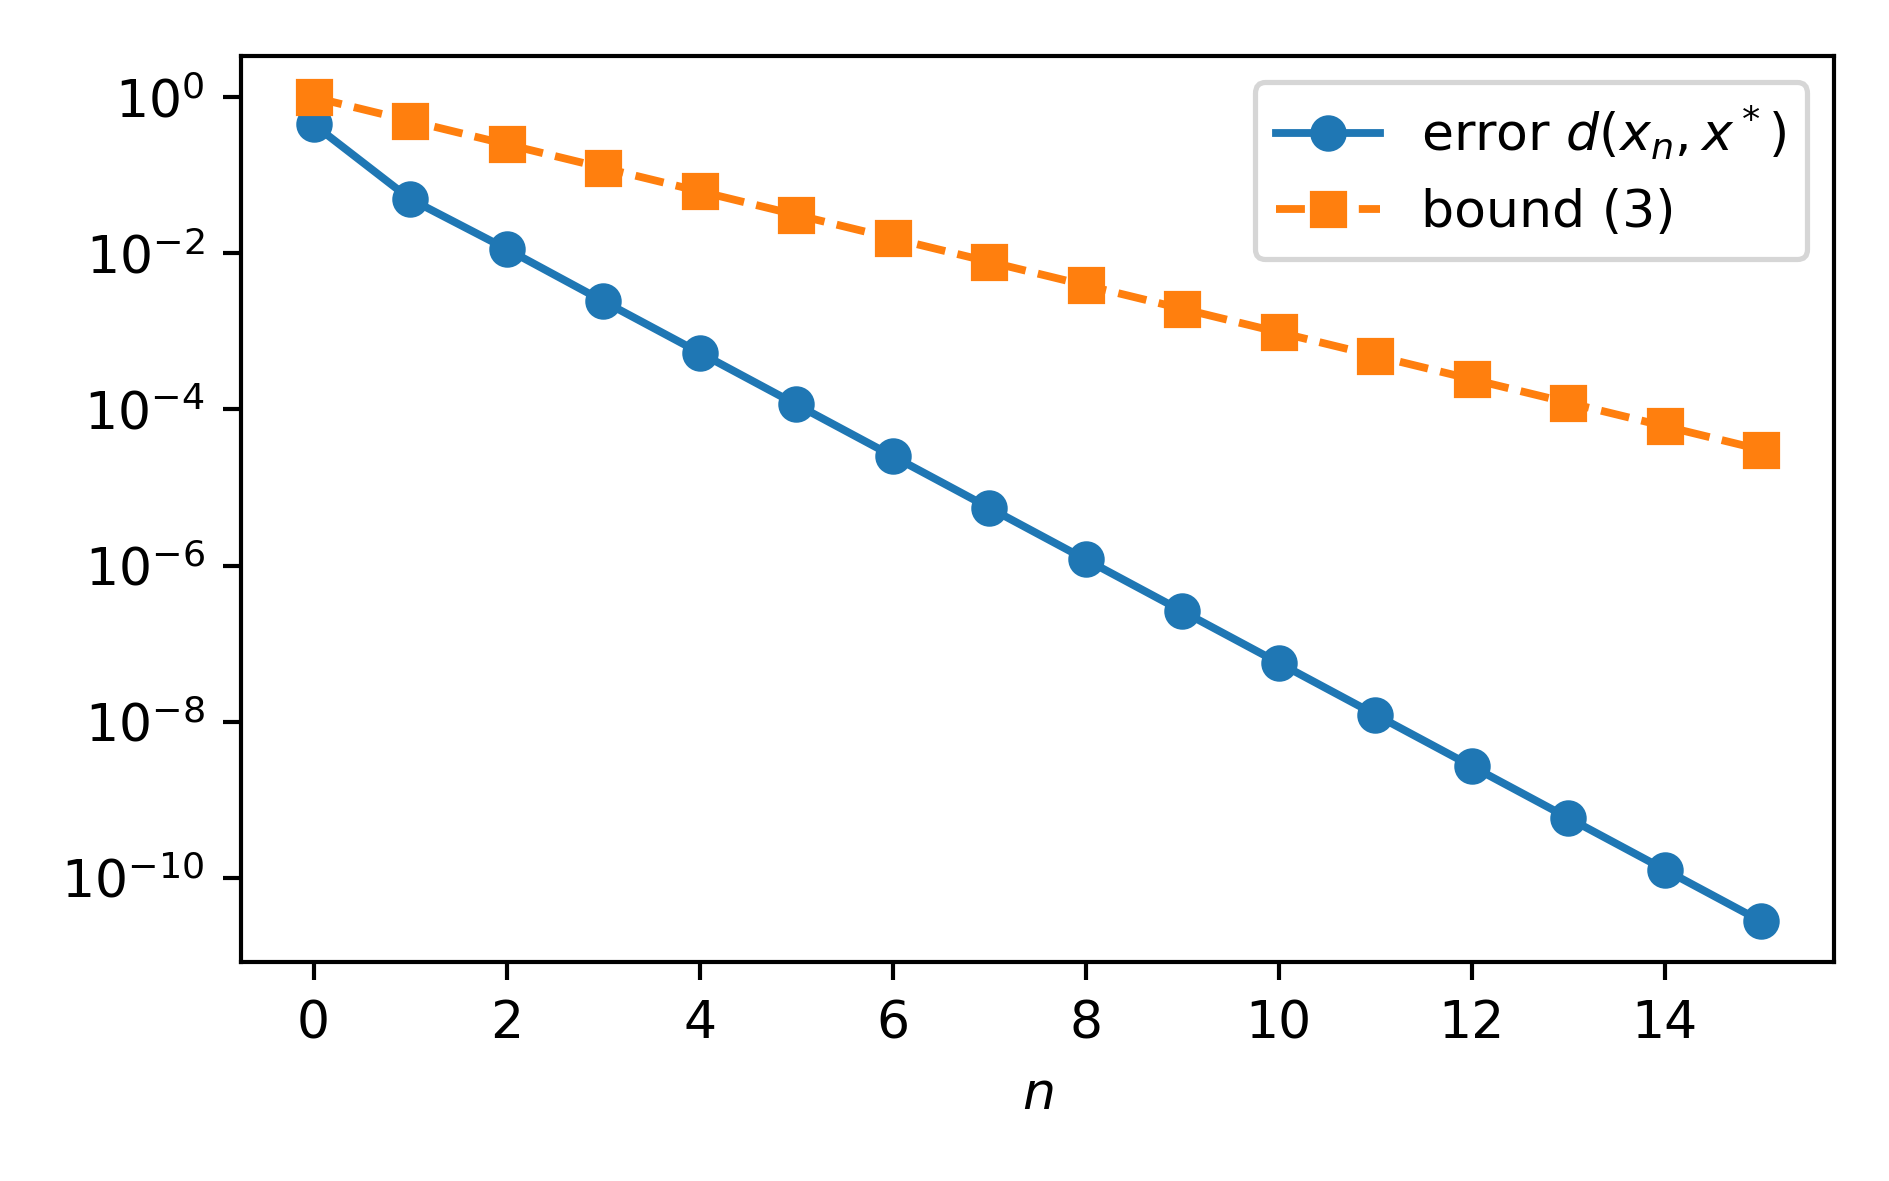
\includegraphics[width=8.0cm]{fig1}
\caption{Error of the Picard iterates for $Tx=\tfrac12\cos x$ and the a priori bound~\eqref{eq:apriori} (logarithmic scale).\label{fig:error}}
\end{figure}

\begin{Remark}
The bound~\eqref{eq:apriori} only uses $q$ and the first step, so the number of iterations can be fixed in advance. Since $|T'(x^*)|=\tfrac12|\sin x^*|\approx0.22$, the actual error decays faster than $2^{-n}$, as Figure~\ref{fig:error} shows.
\end{Remark}

\section{Conclusions}\label{sec:concl}

We gave a self-contained proof of the a priori error bound for Picard iterations of a contraction on a complete metric space and of the resulting stopping rule. The scalar example shows that the bound is reliable but conservative when the local Lipschitz constant at the fixed point is smaller than the global one. A natural next step is a posteriori bounds that use the last two iterates and local contraction constants.

%%%%%%%%%%%%%%%%%%%%%%%%%%%%%%%%%%%%%%%%%%
\vspace{6pt}

\authorcontributions{Conceptualization, I.P. and O.K.; formal analysis, I.P.; software, I.P.; writing---original draft preparation, I.P.; writing---review and editing, O.K.; supervision, O.K. All authors have read and agreed to the published version of the manuscript.}

\funding{This research received no external funding.}

\institutionalreview{Not applicable.}

\informedconsent{Not applicable.}

\dataavailability{No new data were created or analyzed in this study. Data sharing is not applicable to this article.}

\acknowledgments{The authors thank the anonymous referees for their comments.}

\conflictsofinterest{The authors declare no conflicts of interest.}

%%%%%%%%%%%%%%%%%%%%%%%%%%%%%%%%%%%%%%%%%%
\begin{adjustwidth}{-\extralength}{0cm}

\reftitle{References}

\bibliography{references}

\PublishersNote{}
\end{adjustwidth}
\end{document}
